\documentclass[midd]{thesis}

\usepackage{graphicx}
\usepackage{times}
\usepackage{clrscode}
\usepackage{mathtools}

\newcommand{\tab}{\hspace*{2em}}

\bibliographystyle{plain}

\title{He Doesn't Know the Territory\\
\small{An investigation of Heuristics for the Traveling Salesman Problem.}}
\author{TREVOR HARRON}
\adviser{Professor Mathew Dickerson}

\parindent=0in
\parskip=7.2pt
\openup 1.5em

\begin{document}

\maketitle

\abstract{
	\tab The Traveling Salesman Problem (TSP) is the problem of finding the shortest Hamiltonian Cycle of a given a complete graph G? Because finding the optimal solution to the TSP is NP-Complete problem, heuristic approaches are an important part of studying the TSP and has a important role in finding routes in the real world. In this paper, five heuristics, Nearest Neighbor, Greedy, Minimum Spanning Trees, Genetic, and Christofides, are examined on real world state data on not only quantifiable metrics but also qualitative ones but also implemented from scratch. The quantifiable metrics include theoretical and actual runtime and space and if present the upper bound guarantee of the heuristic. The qualitative metrics include the difficulty of implementation and the knowledge required for implementation. The results of the tests on state data show that while looking at the theoretical complexities are a good indicator of how the heuristic can preform it is by no means a definitive guide. 
}

\acknowledgements{
	\tab I would like to acknowledge my advisor Professor Mathew Dickerson for his guidance on this paper and pushing me to work my hardest. Also, I would like to thank Katrina Schweikert of Middlebury's Geography department for her invaluable help with navigating ArcGIS. Finally, my friends, family, and the Computer Science Department at Middlebury College for their support.
}

\contentspage

\chapter{Introduction}
\tab The Traveling Salesman Problem (TSP) is simply the question if a salesman is trying to visit each city given a set of cities once without driving on the same road more than once and ending at his starting location again, what route does he take? In essence for a cyclical graph, what is the shortest Hamiltonian Cycle. More formally, the TSP is defined as given a Graph $G$ is a set of $N$ cities $C$ and a set of edges $E$ such that $e \in E = (c_{i}, c_{j},k)$ where $i \le N, j \le N$ and $i \ne j, c \in C$, and with $k$ as the cost to travel on that path, find the path that covers every city with a minimal cost and returns to the starting city $c_{0}$ in $G$. \\
\tab The TSP turns out to be in a class of problems known as NP-Complete\cite{cai} (due to the NP-Completeness of finding Hamiltonian cycles in 1972\cite{karp}) meaning that computer scientists do not know if a efficient solution exists to find the answer but that an answer can be verified efficiently. The algorithmic complexity of the naive solution where we check every possible route turns out to be $O(n!)$. It is important to note that when I say an efficient solution I mean one that can be solved in a Polynomial amount of time i.e. $O(n^k)$ where $k$ is a constant. Even for smaller instances of the TSP it turns out to be infeasible to use the naive solution for the case of trying to visit every capitol in the United States (starting at Washington D.C.) it would take an inordinate amount of time and processing capabilities to solve. This also means that for the graphs that are being examined the exact optimal distance cannot be known. Even with improvements to the algorithm such as using Dynamic Programming (which is outside the scope of this paper) the complexity is $O(n^{2}2^{n})$\cite{dyn}, which is still not polynomial making it  infeasible to always find the optimal solution. Despite this there is still the need for solutions to the TSP especially with companies such as FedEx and UPS that depend on the quick and efficient delivery of mail and packages to a not fixed set of locations from day to day. In an effort to find other solutions to the TSP computer scientists work on efficient heuristic algorithms that may only find an approximate solution to the TSP. These heuristics are known as heuristics and are the subject of this paper. There are various permutations of the TSP that include the symmetric and the asymmetric TSP, but for the purposes of this paper there is not a distinction drawn between them. Other forms of the TSP that are not part of this examination at all in this is the Euclidean TSP, which does not use the network distances but instead the Euclidean distances (hence the name), the Constant, and the Small TSP, the Bottleneck TSP, Time-Dependent TSP, and the Stochastic TSP. There are some cases where the TSP has also been solved, however, this paper is trying to examine these heuristics with the General TSP generated from real road data.\\
\tab For this project, the graphs that these heuristics will be run on comes from the real set of cities from the continental United States and the edges of the graph are calculated based on the network distance (road distance) in between the cities. Given the in feasibly large number of cities and roads in the United Stats as a whole, the graphs used are created from the cities and roads of a single state (with islands and other non-reachable cities removed) as opposed to using the continental United States as a whole. This paper intends to address the implementation of various heuristics and show that these heuristics can be used in real world scenarios and look at the performance of each heuristic.\\
\tab Most of the heuristics that are examined in this paper are also called Tour Construction heuristics. These are heuristics that are used in the construction of the route and for the most part can guarantee being 2 times the optimal length. It is important to note that a subset of these heuristics are local search heuristics (such as Nearest Neighbor) and those cannot be guaranteed to be within a multiple of the optimal solution\cite{ttps}. Among these heuristics are the Nearest Neighbor heuristic, the Greedy heuristic, the Minimum Spanning Tree  heuristic, and the Christofides heuristic. The second heuristic that will be examined is a family of tour improvement heuristics based on Darwin's Theory of Evolution called Genetic Algorithms. Other Tour Optimization heuristics, Combinational heuristics, Ant Colony heuristics, Approximation heuristics, and Branch and Bound heuristics are not examined in the scope of this paper. In short, the heuristics that are covered in this paper are only a small portion of the possible heuristics in the world of TSP heuristic studies. \\
\tab To test the heuristics, an Experimenter class was created to test each of the solvers multiple times on the various state-based graphs. The results from the various heuristics are recored based on time, memory and distance.  The time is the number of seconds required to solve the graph, the space is in Megabytes needed for space along with the distance of the found route in meters. For each solver, five states were used to create the graphs needed for testing. These graphs, vary in size of the set of cities as well as the number of routes from one city to the next. Each of these graphs with be used to see the overall effects that the size of the graph has on the performance of the heuristics.\\
\tab Before moving on to more details of the heuristics being studied, there is one important concept that should be kept in mind, which is the Held-Karp lower bound. The Held-Karp lower bound is a good measurement of comparison of an heuristics performance. The computation Held-Karp lower bound is ``...the solution to the linear programming relaxation of the integer representation of the TSP'' \cite{htspc}. In short, the Held Karp algorithm used to create the Held-Karp lower bound is a solution using a non-graphical representation of the TSP. This polynomial time algorithm has been found to be within .08\% of  the optimal length in most cases and at worst within $2/3$ of the optimal tour. As such is a reliable metric to use in evaluating heuristics of the TSP. In short it is important to keep this as a concept since it is be referenced several times as a means of algorithmic evaluation.\\
\tab As whole, heuristics have been studied as a potential alternative to the naive solution to the TSP. This pursuit then led to the a conclusion stating that if there was a heuristic that guaranteed an optimal solution there then $P = NP$. For the most  part, computer scientists agree that $P \neq NP$ and as such there is not an efficient solution that will also guarantee the optimal solution. In lieu of that, to investigate the various heuristics of the TSP, several heuristics have been chosen for their algorithmic complexity and guaranteed maximum distances as an example of most of the conventional approaches that currently exist. These heuristics are Nearest Neighbor, Greedy, Minimum panning Tree, Genetic, and Christofides heuristics. Each heuristic is implemented and then tested based on their runtime, their CPU usage and distance of the routes they produce.\\ 
\tab The heuristic algorithms implemented are measured on several different qualities. These qualities include the algorithmic time and space complexity as well as the actual run times and CPU usage and on the guaranteed upper bound of the various heuristics. In addition to those measurements, the heuristics are also be evaluated on the complexity of implementation. The complexity of implementation means the number additional functions needed for the heuristic, the extra data structures, as well and the additional knowledge that the implementer would need. Encompassing some of this complexity is also the additional work needed for the helper functions for the heuristics as well. The complexity of implementation, though mostly qualitative in nature, is examined quantitatively in looking at the amount of time needed for writing each of these heuristics in addition to any comments about the number of lines of codes, the number of class variables, etc. These are then be put through t-tests to see if there are any significant differences in the results in terms of one heuristic's efficiency in the different qualities. These results in combination with the notes on implementation are then be used to see if there are significant improvements that could be made.\\
\tab The implementation of the entire project is in Java. Before moving onto the heuristics, it is important to give a brief description of the basic classes/interfaces used for such a project. The interface most concerned with the graph's construction (apart from the Graph interface) is the Reader interface who's job it is to parse information in either a Comma Separated Value (csv) document or a Key Markup Language (kml) document. As a note: to be able to parse and use kml documents required to construct the graph an external library designed by the makers of the kml format (citation here) was used to read the of all of the cities was used. Readers can also be implemented to take any other number of formats in theory but for the purposes of this implementation kml files and csv files were focused on. The Reader is able to take the documents preprocessed to either csv or the kml formats and translate that into a graph. The different readers that are implemented from the Reader Interface are then used to parse these different formats: csv for roads, csv for locations, and kml for city locations.\\
\tab The Graph interface allows for different representations of the graph to be used abstractly through some key methods. There are some basics that each graph has such as Nodes and Edges to represent the cities and roads. The two graph implementations could used for this were and adjacency matrix model and the list model. The matrix model was used and is defined as a graph represented in an $N$x$N$ matrix, where $N$ is the number of cities, and the edge $c_i,c_j,k$ goes from city $c_i$ to city $c_j$ at a cost $k$ and is at position $(i,j)$ in the matrix such that $i \neq j$. Those edges that are on the diagonal have been declared as $null$ since it is trivial to account for road going to themselves in the implementation of heuristic. The list model has a slightly different structure where the Nodes contains a list of pairs of Nodes and distances from Node to Node and is not implemented in the course of this paper. Due to some of the restrictions of programming languages (and for the sake of simplicity in parsing the data) The Edges of the graph are directed though the for each city pair there is an edge going from one city to the other and visa-versa (this happens to be the case in the instances presented in this paper). In essence, this makes abstracts away from the complicated potential of changing the heuristics for directed roads and non-directed and allows for us to better examine the heuristics themselves.\\
\tab For the Edge and Node classes the implementation is relatively straightforward but critical to the whole paper . For the Edge class the Edge holds the object identifiers for both the city the road is going from, the city the road is going to, and the distance in between the two points. This distance is not Euclidean but is instead based off of the network distance traveled by road to get from one place to the other and is explained more in chapter 2. The Edge class is that it implements the Comparable interface from the Java standard library allowing it to be sorted in the heuristics where sorting of Edges is required. The Node class holds the basic information about the city/point of interest such as the x coordinate, y coordinate, the name of the place, a unique identifier of the location (generally a number and name combination) and the position it was read in the original file. The last variable is to allow for the Node to know where it lies in say a matrix based graph. \\  
\tab The final and arguably most important interface to mention is the Solver. The solver interface is implemented by each of the heuristics tested in the paper. There is also an AbstractSolver class that each of the solvers inherits from to use repeated variables and functions. Each solver sub-class is the implementation of a heuristic approach. These are all created by a factory to help better abstract away from the direct implementations of the solvers. This is used by both the Experimenter class (used for the running of experiments) and for the TSPApplet which is the GUI for viewing the results of the various heuristics. For each different heuristic, there is a solver that goes with it. Also for purposes of clarity in the Java code, the helper functions of the heuristics are not displayed as that would clutter the examination of the algorithms (except in certain cases where they are the defining factor of the algorithm's time and or space). Each solver also uses the necessary classes to solve the problem and methods that go along with that; for example a Minimum Spanning Tree Solver (or MSTSolver) would contain a Tree object and the method for transversing the tree. These more specific cases are described more detail in chapter 3. For purposes of clarity, the result of the solver is an ArrayList (re sizable array) of the cycle of cities, the distance of that cycle as well and the time, and space used to solve the graph. Testing has been done to ensure the accuracy of the heuristic's implementation, the accuracy of the solution on a small (less than 10 cities) dataset as well as the durability of the code in place. This dataset has no bearing on an place in reality and as such is not considered in the analysis of the heuristic algorithms.\\
\tab The final set of classes that should be discussed are the ones pertaining to the visualization and testing of the project. These classes are pretty self explanatory and focus on using the Readers to create the graph and the Solvers to solve it. In the terms of the differences between the Experimenter and the TSPApplet, the Experimenter finds the solution and repeats the experiment a certain number of times adding the results to a csv file to be analyzed with t-tests or to use for graphic representations of the results. The TSPApplet is a Java applet whose purpose it is to view the results of a single iteration of the the solver for a given graph. The graph and the solver can both be chosen by the user to allow for easy viewing of the heuristics of the TSP. Overall, the need for these classes is paramount to the study, analysis and debugging of the heuristics implemented in this paper.\\
\tab As a final note, the code was written with good usable practices in mind. As a result of this, the code developed was tested incrementally on the small data set and tried to use elements of good Object Oriented design. The classes are in packages appropriate to their function, names either are intuitive or were named to mimic the pseudo-code (for readability in side by side comparisons), inheritance was used as a means of preventing rewriting and Interfaces were used in order to abstract away from implementation dependencies. In short, the code developed in the course of this paper was made to try and match industry standards given that there is a strong undertone usability of various heuristics in a space where a trade off must be made in between efficiency and accuracy in the real world.\\
\tab The TSP is a difficult problem to solve and as such the heuristic algorithms are used to approximate the solution are the main focus of study. The various heuristics are implemented in Java as well as the testing, visual, and other necessary parts to creating the graph. The data is based off of real world data and as such the coding practices used focus on real world implementing of these heuristics. In lieu of this the focus of this paper lies not only in the algorithmic time and space but also in the complexity of the implementation as well.

\chapter{The Data and Methodologies}
\section{The Data}
\tab The data used for this project was a combination of road census data for the edges of the graphs and their costs. The road and city data are from the 2006 United States of America (US) census and as such it should be noted that the main use of this data is to show some of the practical applications of the algorithms that are implemented in the course of of this paper. The scope of this data is examined as well as the contents and implications that this may have on the paper as a whole. While this is not critical to the algorithms or the overall results of the paper it is important to examine the data in detail to better to understand the paper as the whole.\\
\tab The cities (or vertexes) are from US census data, which is comprised of the major towns and cities in each of the states and protectorates.  Each of these files were originally in a format called a shapefile a format used by GIS software and contains the geometric data for the objects. These various features include an unique identification number, the geometric shape of the objects, relevant information regarding the geometry, the coordinates of the object, its name, and other pertinent features. While shapefiles are useful for GIS studies the format is not parsable for the purposes of this paper.\\
\tab For the city shapefile, the geometry was simply a point with the coordinates for the point on the latitude and longitude. The cities also have a name and a state that they are a part of, the basic information including the city's id and other information such as population size, range, and the county that the city is a part of. The cities however do not contain road data, the road data is contained in a different shapefile.\\
\tab The roads are a set of several different segments, arcs, and junctions forming complete paths. It is important to note that these required some additional preprocessing to ensure continuity in certain cases but the distances were not affected by this. For the distance data that each segment has is in meters and additional distances used meters to avoid conversion errors. The overall distances between the cities then use the distances of each of the segments to find the distance from one city to the next.\\
\tab There are two different kinds of raw data that are used in this paper, one that contained the cities and one that contained the roads. Both of these were originally in shapefiles and had to be preprocessed for implementation of the graphs. Despite the extra steps the benefit of the shapefile format is the meta-data that it contains both in terms of content and with geometric data. Some of this meta-data is useful for the purposes of this paper especially the geometric data in particular. The combining and binding of the two different sets of data occurred in the graph creation after the data preprocessing.

\section{Data Preprocessing}
\tab To gather the data, US Census city data from 2006 was used to for the cities and from 2013 for the roads in the US and per-processed using ArcGIS. The set of cities was saved from its original shapefile format to a readable format called kml (Key Markup Languages) which maintained all of the spatial and geometric properties of the original format. These properties include the state that the city resides in, the coordinates of the city, and additional properties that a user might useful. These features are the ones that are in the shapefile previously mentioned. To transfer the shapefiles into the more readable kml and csv file formats was the tool ogr2ogr (pronounced ``Oger to Oger"). Ogr2ogr is a open source tool whose sole purpose is to `'translate" shapefiles to other formats. These formats range from other GIS formats like raster,  geojson (a variety of json), kml, csv and more. Among these formats there was research done as to what the best format to use for both the cities and the roads before choosing the final formats to store and parse the data in.\\
\tab Before even considering translating the formats into a parsable format the data needs to be processed from its raw form into the graphical form that is used. Then to calculate the network distances of each city, ArcGIS was used. To gather the distances first in ArcGIS is that an OD Cost Matrix was created from the cities of a given state and all of the roads from the census data. Naturally, to ensure that there are not any errors that occurs from the preprocessing that ArcGIS does in laying down roadways on the map there was some manual labor involved in ensuring the roads that are supposed to connect to each other do. Such errors can occur due to slight miscalculations in the data itself or in how the shapefiles are processed in ArcGIS. The corrections that occurred include the connection of roads that are continuous, the linking of cities to the closest road, and even telling the OD Cost matrix that  some roads end at the coastline away from cities and should not be considered. In the creation of the OD Cost Matrix the cities are filtered by the state that is being used in the creation of the graph for the vertexes. All of these edges are placed as the origins and the destinations of the matrix to try and find all of the edges for the graph that are possible. To ensure the completeness of the graph and that there are not any disconnected cities, the cities that are on unreachable locations such as islands were removed. Such features would also make several of the algorithms infeasible.\\
\tab The Reader class is primarily responsible for parsing the various formats and converting it for the uses within the Graph. In terms of the implementations, the classes for reading the kml and the csv formats are distinctive to what the data is used for. For instance the KMLReader reads the kml file of cities and uses the meta-data to create the cities for the graph to hold. With the CSVReader, the initial implementation meant that the roads were the only part to be read but this could easily be changed to accept arbitrary locations of interest to visit as well as the edges. To ensure that the algorithms and parsing work correctly, there is also a sample dataset that have been created consisting of five vertexes which are interconnected by edges with costs. This ample data uses the same formats as the actual data.\\
\tab For the distances and edges, ArcGIS uses a variant of Dijkstra's algorithm\cite{gis}. These distances were then stored in line objects that consists of an id, a pair of cities in the form of `'to - from" and ending in the distance of the route. All of these line objects were then stored in a shapefile tied to the OD Cost Matrix. To read these lines the shapefile takes from export it and then translate it into a csv file. In the case of a csv file there is not the geometry of the lines at all. This lack of geometry is not of concern however since the lines are tied to the cities meaning that the geometry of the lines is not needed at all. In fact the only line geometry that is regarded is the lines that are stored in the roads which has been mentioned before. For the lines that are then represented in the graphics are represented as a straight line instead of the network distances. This is purely for the ease of displaying the graph as a whole.\\ 
\section{Methods}
\tab The methods used for testing are very simple in terms of concepts needed. The information that is being gathered is simply the amount of time needed to run the algorithm, the space, and the distance of the route that the algorithm produces. To gather all of this extra data, it is simplest to gather it when obtaining the result, which is simply an array of the order of cities are visited in to get the route. Of course also to gather this information there is extra code that has been added to the algorithms which have no effect on the result itself nor its time or space usage in any significant way and of course have no impact on the algorithmic evaluations.\\
\tab To gather the time that it took a given heuristic to run, Java has some built in features to help keep track of the time an operation was started which is the basis for the time keeping that is used. Admittedly, the fully time keeper is gathering the starting time then immediately after the program is complete gather the ending time, and then find the difference between the two and converting it into a readable format. The amount of time is recorded in the final solution in terms of seconds. For the smaller datasets concern is understandable for the purposes of measuring time some might find the use of tenths of seconds more useful but for the larger cities examined, it would soon become clear that seconds is not only valid but easily puts the results in context without meaningless conversion. The amount of time that it takes the program to run is the first of measurements to be added to the result.\\
\tab As stated in the introduction, since Java is used as the language of implementation, gathering memory usage is not a straight-forward matter. However, to be able to look at the memory usage, all that is simply done is use a function that calls Java's garbage collector and then look at the total memory and free memory to see how much was used. The function called is `'System.gc()'  for `Garbage Collection'. This technique is frequently used in programs to check for memory leaks (i.e. data that is not cleaned up properly. The calls to get the used amount of memory and the total memory are System.totalMemory() and System.freeMemory(). By finding the difference in the two we can find the amount of used memory there was. However, also as mentioned earlier, the memory is being collected in terms of Kilobytes (KB) so the difference is then divided by 1024 (since 1024 bytes go into a KB). To avoid any issues this might have on the time, the space is taken after the time is taken. This number of KB that is used is also then added to the result that is returned.\\
\tab Distance is the final quantitative measure that the heuristics are being evaluated on. The distances themselves come from the road distances calculated as mentioned earlier in Data Preprocessing. The gathering of distance occurs at different times depending on the heuristic in question but are either gathered during the construction of the route or after the route has been constructed. For the gathering of the distances during the tour's construction, the distance is only aggregated after it has been confirmed that a route from one city to another has already been added to the final tour produced. Also, for each of the tours it is needless to say that the final distance back to the original starting city has been included in the final distance.\\
\tab To evaluate the code and the heuristics overall there are two main forms of evaluation, quantitative and qualitative. It is simple enough to understand the quantitative measures, these are based on the use of time and space and are measured in terms of big-O notation. In addition to the algorithmic time and space the actual time and space and distance result of the algorithm are also measured. The quantitative approach for evaluation is the number of extra helper functions and the algorithmic complexity and implementation of these functions. The qualitative approach to the heuristics comes from looking at the knowledge required to implement these algorithms. This is a qualitative measure given that this information while measurable in terms of number of concepts, does not lend itself to more definite measures. More of the qualitative measures also include the intuitive difficulty of the heuristics in both understanding the approach itself as well as the intuition of the implementation. The quantitative measures of the algorithms are then confirmed as different ranging from heuristics to heuristic with t-tests to show if there are significant differences between the results of the algorithms. In conclusion, the methods for evaluation are both quantitative and qualitative and for the most part, there are many attempts of quantify all of the data.

\chapter{Heuristics}
\section{Introduction and Conventions of Pseudo-code}
\tab The purpose of Heuristics chapter is to explain the heuristics of this paper and some of the benefits and detractions of each approach. This discussion includes the algorithmic time and space, guarantees,  additional functions, data structures, and algorithmic concepts. The complexities of implementation are also discussed in this chapter.\\
\tab The pseudo-code used in this paper does not conform to a single set of per-defined conventions but  still attempts to be as readable as possible. This includes the use of plain English and mathematical symbols to concisely give the algorithm in a readable format. Plainly named, black box functions have also been used to help show the functions needed for the heuristic. The pseudo-code also appears in a more Object Oriented approach to better show connections between the pseudo-code and the Java code.
\section{Nearest Neighbor}
\tab One of the simplest heuristic algorithms is a greedy approach called Nearest Neighbor (NN). This heuristic's approach is to first start at a random city (or a specified city) look locally at the cities nearby and then adds the closest unvisited city to its to the solution. Then second keep adding cities in this method until there are no cities left and then finally find and add the edge back to the starting city. This is a local and greedy approach to solving the TSP. It is to be noted that while in some cases the cost of the algorithm is taken after the route has been found but for this implementation of nearest neighbor the distance of the route is taken when the city is added to the route. The pseudo-code for the algorithm briefly described above is shown below:\\
$\proc{NNHeuristic}(G)$:
\begin{codebox}
\li $U \gets getStart(G)$ //random start city
\li $V \gets getCitiesExceptStart(G)$
\li\While $V$ not empty:
\li $u \gets$ most recently added vertex to $U$
\li Find vertex $v \in V$ with smallest cost $u$
\li $U.add(v)$
\li $V.remove(v)$\End
\li $findRoute(U, getStart(G))$
\li\Return $U$
\end{codebox}
And below the Java equvilent:\\
$\proc{public ArrayList$<$String$>$ solve}()$\{
\begin{codebox}
\tab//Initializing variables\\
\tab long startTime = System.nanoTime();\\
\tab long seed = System.nanoTime();\\
\tab Collections.shuffle(V,new Random(seed));\\
\tab U.add(V.get(0));//random start
\end{codebox}
\begin{codebox}
\tab V.remove(0); double distance = 0.0;\\
\tab\While(!V.isEmpty())\{//The algorithm\\
\tab\tab String u = U.get(U.size()-1);\\
\tab\tab Edge e = findMinVertex(graph.getCity(u),graph);\\
\tab\tab graph.setRoadVisited(true,e);\\
\tab\tab String nextCity = e.getTo();\\
\tab\tab distance += e.getDistance();\\
\tab\tab U.add(nextCity); V.remove(nextCity);\\
\tab\}\\\End
\tab Edge road = findRouteToStart(U);\\
\tab U.add(road.getTo());
\end{codebox}
\begin{codebox}
\tab distance += road.getDistance();\\
\tab U = getMetrics(U,startTime,distance);\\
\tab \Return U;\\
\}
\end{codebox}
As the runtime of this algorithm is $O(n^2)$\cite{htspc} with a space complexity of $O(n)$. This approach in most cases though the results are typically within $25\%$ of the Held-Karp lower bound\cite{htspc}. However, there is not a guarantee for there to be a upper bound that is a multiple of a constant $k$ of the optimal route. This is not optimal in terms of the distances the algorithm produces.\\
\tab As you can see the implementation of Nearest Neighbor is relatively simple and only requires a few additional helper functions including findMinVertex() and\\ findRouteToStart(). For the purposes of focusing on the algorithm these functions are not shown above. Theres is no additional knowledge required for this implementation aside is how to use of a loop making this a very simple approach. With this in mind it is nice to have a simple implementation of such an algorithm that can find some approximate solution very quickly. An additional part to keep in mind is that depending on the starting city for the tour (which is random) for the simplicity and testing purposes of the implementation, it is possible for several different routes to be produced. With a small change, the implementation could be altered to accommodate a specified starting city. \\
\tab It should be noted in the data that the actual route and distances vary in both terms of the cities to be visited and in terms of the distance that it takes to travel. This while not ideal in terms of having a reliable answer is not necessarily an impairment to the approach as a whole. The reason for this logic is that the algorithm could be run multiple times keeping track of the most efficient route found and returning that. In terms of the heuristic itself its benefits are that it is the simplest algorithm in terms of the concepts needed for the implementation as well as the amount of code for the implementation itself.

\section{Greedy}
\tab The second tour construction heuristic algorithm that is being examined is also a greedy approach similar to the Nearest Neighbor algorithm but is called the Greedy heuristic. As the name suggests the Greedy heuristic uses a Greedy approach to construct the tour of the traveling salesman. The idea is simple, sort all of the edges and use the shortest edge to construct the tour as long as you don't raise the degree of the vertexes more than two and that the edge doesn't make a cycle of less than $N$ where $N$ is the number of vertexes in the graph. The pseudo-code for the algorithm is displayed below.\\
$\proc{GreedyHeuristic}(G)$:
\begin{codebox}
\li $E \gets G.getRoads()$
\li $sort(E)$
\li $R \gets []$
\li $N \gets$ number of Vertices in G
\li\While $R.size <= N$:
\li $r \gets E[0]$
\li \If r does not makeCycle(G, r) and does not raiseDegreeMoreThan2(G, r)
\li R.add(r) \End 
\li remove r from E \End
\li\Return findRoute(R)
\end{codebox}\
The Java implementation:\\
$\proc{public ArrayList$<String>$ solve}()$\{
\begin{codebox}
\tab//Initializing variables\\
\tab long startTime = System.nanoTime();\\	
\end{codebox}
\begin{codebox}
\tab ArrayList$<$String$>$ result = new ArrayList<String>();\\
\tab//sorting and ensuring there are no duplicates\\
\tab Collections.sort(roads);\\
\tab maxEdges = graph.getCities().keySet().size();\\
\tab route = new ArrayList$<$Edge$>$();\\
\tab//finding the route\\
\tab int numEdges = 0;\\
\tab\While(numEdges $<$ maxEdges)\{\\
\tab\tab Edge road = roads.get(0);\\
\tab\tab \If(!moreThanTwoDegrees(road,route)\\
\tab\tab\tab \&\& !makesCycleLessThanN(road, route))\{\\
\tab\tab\tab pathGraph.addEdge(road);\\
\tab\tab\tab route.add(road);\\
\tab\tab\tab numEdges++;\\
\tab\tab\}\\\End
\tab\tab roads.remove(0);\\
\tab\}\\\End
\tab //obtaining the result\\
\tab double distance = findRoute(result, route);\\
\tab //final preparing of the data\\
\tab result = getMetrics(result,startTime,distance);\\
\tab \Return result;\\
\}
\end{codebox}
\tab As can be seen above this is also a conceptually simple construction heuristic based of the theory that using the shortest edges help create the shortest route. However, like Nearest Neighbor, this algorithm has no guarantee of a upper bound on the distance returned though the Greedy algorithm averages within 15-20\% of the Held-Karp lower bound\cite{htspc}.\\
\tab Before moving forward with the analysis of this solution, it should be noted that there are two different graphs here. The first (named graph) is similar to the Nearest-Neighbor approach and is simply is the graph that the solver is working with. The second graph, named pathGraph, is a graph to help simplify the process of adding edges to the route and the functions makesCycleLessThanN() and moreThanTwoDegrees(). These functions each take $O(n)$ time in the worst case scenario. The check for making a cycle is simply an iterative linear-search since the graph used (the pathGraph) only has the set of roads in the route making checking for a cycle simply going from one node to the next and seeing if we have seen it before. The process of checking if an edge would increase the degree to be greater than two relies on the pathGraph to count the instances of Edges and if for a Node there are more than two edges going into it and from it. This means that the overall runtime of the algorithm is at most $O(N^2)$ where E is the number of Edges that the graph has. Now I say this in the instance that there is no guarantee that in the number of cities N a solution will be found but in iterating over the Edges we find the solution doing $O(N)$ work from the previously mentioned functions for each Edge. Sorting of the edges is done int $O(N\log N)$ time and thus in this case is $O(E\log E)$ time and $O(E)$ space used. Therefore the entire algorithm runs in $O(ElogE + N^2)$ or $O(N^2)$ time and $O(E+N)$ space.\\
\tab From this approach a few things are especially relevant, the first is that the Greedy heuristic is deterministic. This provides for consistency in the path that might be desirable in some instances. The amount of overhead knowledge that is required by this algorithm is also very small, all that is required for the helper functions is some knowledge of graph theory with some simple algorithms related to finding cycles. If you are also constructing the actual graph (as was done above) then this task become simpler to accomplish. Overall, this is a simple algorithm to also implement but it should be no surprise that the developer would need to not only have the Edges implement a comparable interface but also ensure that the destructive behaviors of the algorithm do not affect the graph as a whole.

\section{Minimum Spanning Tree}
\tab The final construction heuristic that this paper examines is the Minimum Spanning Tree heuristic. The basic approach is to using the graph make a minimum spanning tree and then create the tour from a preorder transversal of the tree. For some explanation, a minimum spanning tree is an acyclic graph (tree) connected to all of the vertices with a minimum cost. This is a more complex heuristic since some people would not think of creating a tree as a step to creating a cycle. The deceptively simple pseudo-code for the approach is below:\\

$\proc{MSTHeuristic}(G)$:
\begin{codebox}
\li T $\gets$ make a MST of G
\li \Return the depth-first transversal of T
\end{codebox}
This is more complicated in practice as seen in the Java Implementation:\\
$\proc{public ArrayList$<String>$ solve}()$ \{
\begin{codebox}
\tab long startTime = System.nanoTime();\\
\tab ArrayList$<$String$>$ V = new ArrayList<String>();\\
\tab \For(String v: graph.getCities().keySet())\\
\tab\tab V.add(v);\End\\
\tab long seed = System.nanoTime();\\
\tab Collections.shuffle(V,new Random(seed));//random start\\
\tab//make the Tree\\
\tab Tree mst = makeMST(V.get(0));\\\\
\tab//get the result\\
\tab ArrayList$<$String$>$ result = mst.treeWalk();\\\\	
\tab//get the metrics\\
\tab result.add(result.get(0));\\
\tab double distance = getRouteDistance(result);\\
\tab result = getMetrics(result,startTime,distance);\\
\Return result;\\
\}
\end{codebox}
\tab As stated before, this approach involves more complex algorithms than in the previous approaches. First of all this involves the makeMST() function. For the purposes of this paper, the algorithm used was based off of Primm's MST algorithm. Primm's MST algorithm is a greedy algorithm, and with the implementation of this algorithm, there is a slight difference with the original algorithm. The original algorithm uses a data structure called a heap used as well as an adjacency list for the graph so it runs in $O(E\log N)$ time, but the implementation that is used collects the edges on the frontier and sorts them. While this takes $O(NE\log E)$ time, it is a slightly simpler implementation then the use of a heap and exacting the values no longer applicable from it when the frontier changes. The time $O(NE\log E)$ also is the upper bound time for this algorithm since the transversal of the tree takes $O(N)$ time since an iterative pre-order to save space on the virtual stack uses an iterative traversal.\\
\tab The benefits to this heuristic is that there is a guarantee of a upper bound on the distance that the route produces of 2 times the optimal route. This is a nice change from the other heuristics that might have better run times because the other algorithms explained thus far do not have a guarantee making them potentially impractical for real time use. The second benefit is that if there are data structures and functions already in place that can be used such as a Tree, the function to make the MST, and the tree transversal function, then the actual code necessary is unbelievably straight forward (as seen in the pseudo-code). However as was said before there were a fair number of additional classes that were created so that this function was possible which make the implementation more complex than the previous heuristics.

\section{Genetic Algorithms}
\tab The only tour optimization heuristic that this paper examines is the popular family of algorithms called genetic algorithms. These algorithms mimic the evolutionary process by having a population, a fitness characteristic, a breeding mechanism, and a chance at mutation within individuals. The basic concept is to implement each of the characteristics and at the end of a number of iterations pick the fittest example as the result. The pseudo-code for the algorithm helps show this approach below:\\
$\proc{GeneticHueristic}(G)$:
\begin{codebox}
\li V $\gets$ G.vertices()
\li population $\gets$ several random orderings of V
\li \For $k$ times:
\li find the best canidates from population
\li breed those candates
\li randomly mutate some of the offspring \End
\li \Return the most fit member of the population
\end{codebox}

And the Java implementation below:\\
$\proc{public ArrayList$<String>$ solve}()$\{
\begin{codebox}
long startTime = System.nanoTime();\\
\tab ArrayLis$<$ArrayList<String$>>$ population =  makePopulation();\\
\tab\For(int k = 0; $k < 500;$ k++)\{
\end{codebox}
\begin{codebox}
\tab\tab ArrayList$<$ArrayList<String$>>$ parents = darwinsTheory(population);\\
\tab\tab population = breed(parents, population.size());\\
\tab\tab population =  mutate(population);\End\\
\tab\}\\
\tab ArrayList$<$String$>$ result = findBest(population);\\
\tab double distance = getRouteDistance(result);\\
\tab result = getMetrics(result,startTime,distance);\\
\Return result;\\
\}
\end{codebox}
\tab This is a tour improvement heuristic focusing on trying to find the best route by combining aspects of the shortest routes. This is clearly not a singularly definitive approach to this problem. To clarify some of the finer points of the of the implementation. The first is that the initial population is simply a list of randomly made routes with the restriction that there are no two routes in the original population. This is to better increase the chances that the heuristic will produce a good route. The second thing to focus on is the breeding function. What is implemented is called a moon breeding. With this approach, $2/3^{rds}$ of the first parent is used and then the rest is filled in with the remained cities from the second parent. This is done for every pairing of the best candidates before mutations can take place. The number of mutations and chance of mutation are also both random, allowing for at least 1 mutation to potentially take place.\\
\tab In looking at this approach it is clear that there is a good chance for a good route to come out of this heuristic. The main issue lies in the fact that there is no guarantee of a decent result coming from this approach. In addition, the time it takes to run this heuristics is $O(kN^2)$ where k is a non-negligible constant. In short this heuristic has the potential to preform well but also does not make any guarantees of it's performance making it a good approach if you have an initial population of decent routes but not optimal.

\section{Christofides}
\tab One of the most complicated heuristic algorithms is the famous Christofides heuristic. The approach of this heuristic builds off the concepts of the MST heuristic by first building a MST. Then second find all of the nodes with odd degrees and create a set of minimum pairs with those nodes. Then create a new graph that is the union between the MST and the new set of minimum pairs. Then find the Euler Cycle (a path that visits each of the edges once) of the new graph and take shortcuts if we have visited the node before. The pseudo-code for the algorithm described above is shown below:\\
$\proc{ChristofidesHeuristic}(G)$:
\begin{codebox}
\li $MST \gets makeMST(G)$ //random start city
\li $oddNodes \gets MST.findOddNodes()$
\li $MinPairs \gets findMinPairs(oddNodes)$
\li $G' \gets UNION(MST,MinPairs)$
\li $cycle \gets findEulerCycle(G')$
\li\Return $takeShortCuts(cycle)$
\end{codebox}

and the Java Implementation below:\\

$\proc{public ArrayList$<String>$ solve}()$\{
\begin{codebox}
\tab long startTime = System.nanoTime();\\
\tab ArrayList$<String>$ V = new ArrayList<String>();\\
\tab \For(String v: graph.getCities().keySet()) \\
\tab\tab V.add(v);\\
\tab long seed = System.nanoTime();\\
\tab Collections.shuffle(V,new Random(seed));//random start\\
\tab //make the Tree\\
\tab Tree mst = makeMST(V.get(0));\\
\tab ArrayList$<String>$ oddNodes = mst.getOddNodes();\\
\tab ArrayList$<Pair<String,String>>$ pairs = getMinimalPairs(oddNodes);\\
\tab eulerGraph = unionWithTree(pairs, eulerGraph);\\
\tab ArrayList$<String>$ cycle =  eurlerCycle(eulerGraph, V.get(0));\\
\tab ArrayList$<String>$ result = takeShortcuts(cycle);
\end{codebox}
\begin{codebox}
\tab double distance = getRouteDistance(result);\\
\tab result = getMetrics(result, startTime, distance);\\
\tab \Return result;\\
\}
\end{codebox}
\tab As one can see here, the basic layout of the heuristic is relatively straightforward. The complexities arise however upon the inspection of the helper methods. The various methods needed include finding the Minimum Spanning Tree (with the added part of adding the edges of the Tree to a graph), finding the nodes of odd degree, finding the minimum pairs, finding the Euler Cycle, and taking shortcuts to find the final route. As a result of these methods especially the findMinimumPairs the runtime of Christofides heuristic is $O(N^3)$. The space taken up by this heuristic is similar to the others in that it takes $O(N)$ space to hold the MST and new graph. \\
\tab However, with this trade off of extra time, there is a guaranteed upper bound of any route produced by Christofides to be at most 3/2 times optimal route. This is better than the MST heuristic that has an upper bound of 2 times the optimal length and the other heuristics mentioned that don't have a upper bound. All of that being said, the complexity of implementing this algorithm is non-trivial and neither is the knowledge required to implement it. The complexity comes from the use of several extra functions needed to  complete the heuristic. The second aspect required the might be a limitation for implementing this heuristic is there is a higher level of knowledge required and the code is more complex.

\chapter{Possible Improvements}
\tab For each heuristic, there is some improvement or improvements that could be examined. Some of these include the implementation of the helper functions while others address more complexities of implementation in general. The set of possible improvements can be addressed in a few categories: overall changes, alternative helper functions/implementations, and the complexities of implementation. The overall changes that are going to be described include the placement for the declaration of variables, some common trends that are prevalent in the implementation of the heuristics, and some of the questions surrounding the implementation. The alternative helper functions goes into detail about the various implementations that were used and the various alternatives that could have been implemented instead. Finally, the difficulties in implementation includes all of the various choices that were faced in the course of implementing a heuristic. These categories reflect the challenges that one would face in implementing the heuristics described and provides for potential future work in the study of implementing TSP heuristics.\\
\section{General Improvements}
\tab This paper's code that was produced attempts to implement the best practices for reusable code, but is not perfect. The algorithms and heuristics were written with both ease of implementation and for the accuracy of the result in mind. This means that while the implementations may not be the most efficient they do maintain a high level of accuracy. As such, the practices of declaring variables within loops instead of out of, not using built in iterators, or the creation of new data objects are all examples of sacrificing space for the sake of ease of implementation. Another point that should be addressed is that the implementations are all in Java which has the ability to be run on any platform but is not necessarily the most efficient. In short, there are minor improvements that could have also been made in addition to large algorithmic or implementation changes.\\
\tab There are also other forms of representing a graph that could be used instead of the matrix model that was mainly used. Other forms would be using list of the edges going from a node and the use of actual node edge structure. Another item to note is the representation of the Edge  class. The edges are also directed, making some of the algorithms more complex. This directed nature was circumvented by simply using two edges to represent a singular edge and the algorithms that required undirected graphs then took this into account. This issue arose from the use of a class to represent an edge and by the constraints to make the class consistent. If one were to optimize this they might use more traditional methods for representing graphs without the use of classes for the nodes and edges. Finally, as a trend in the implementation of the heuristics is the extensive use of HashMaps. This is not necessarily a problem with the implementation but it does mean that it is the only way to implementation.\\
\tab For several of the heuristics there are helper functions that were crucial to the implementation of the heuristic, for instance the MST algorithm for the Christofides and MST heuristics. There are several different algorithms that could have been implemented but in the interest of time only one was implemented. Here the specific questions that could arise from examining the code for this paper is addressed in the order that they were discussed in section three. As a common thread for the need for improvements it is safe to assume that most improvements could and would be made in an environment with more people working as a team and a singular approach chosen instead of five. As the more complex heuristics are examined there are more questions that have to be addressed. For the sake of sticking to the point the key functions or concerns about the approaches will be examined and not necessarily every detail of the implementation.\\
\section{Nearest Neighbor and Greedy}
\tab For the Nearest Neighbor and Greedy heuristics there are not a lot of specific improvements. These improvements includes the use of declaring variables outside of the loops for example. Also it is worth it to note that the Edge and Node classes helped ease the difficulty of implementation. For the Greedy heuristic the choice to use an extra graph for the sake of simplifying the algorithms for checking a cycle and the degrees of nodes. This choice meant that there was a increase in space usage that is needed though overall space complexity of the algorithm stayed the same. Typically, checking for a cycle in a graph uses a breadth-first search instead of the implementation which took advantage of the extra graph and used a depth-first search. This choice was made to simplify the overall implementation and draws on the choice to use a second graph in the Greedy heuristic. The second item that could be improved is when counting the degree of the nodes in the graph. The implementation that is used relies extensively on the use of HashMaps instead of checking the each of the nodes in the graph and counting the edges. For the purposes of making improvements to the approaches there are only a few optimizations in general that could be implemented to help the efficiency of the heuristics discussed in the overall comments on implementations. It is simple to see that the heuristics do not necessarily have for lack of better terms less moving part and the number of improvements mimicked it.\\
\section{Minimum Spanning Tree}
\tab Naturally, the third heuristic that needs to be examined is the MST heuristic and the two different algorithms that could be used for the construction of the MST. There are two different algorithms that could have been used Primm's algorithm and Kruskal's algorithm. The difference between the two comes from the implementation and the subsequent run-times of the algorithms. A variant of Primm's algorithm was used for the purposes of this paper for the ease of implementation. This heuristic could simply be improved by the use of a priority queue (or min-heap) instead of the use of an ArrayList that is constantly being sorted. The use of a priority queue allows for the sorting to happen during the insertion and removal instead of explicitly sorting at each step. The use of Kruskal's algorithm could also improve the runtime but would mean that a whole new data structure would have needed.\\
\tab After examining the creation of the MST it us only natural to examine the use of the transversal for the MST heuristic. This comes because the lack of specificity in the description of the heuristic's approach. The approach only specifics that the heuristic uses a depth-first transversal. This leads to three different approaches on how to implement the heuristic: in-order, pre-order, and post-order. After some experimenting with the various transversal algorithms, pre-order was determined to be the most efficient since it arguably better maintains the relations between the various cities as they are added to the route in the creation of the the MST. In-order transversal algorithms work well with the exception that the various edges were added to the MST in the order of the shortest to the longest while a in-order transversal may not maintain this property. Finally, a post-order transversal could also maintain the property in the creation of the MST however was not implemented for the sake of readability. Finally, these transversal algorithms could have been written iteratively or recursively but for the sake of not causing stack overflow an iterative approach was used instead of the recursive approach. These choices for the MST heuristic could be examined in more detail in a different paper.\\
\section{Genetic Algorithms}
\tab To cover all of the possible variants of the Genetic algorithm that could have been implemented is well outside the scope of this paper unfortunately. What can be explained in further detail though is the logic following the approach that was implemented in the course of this paper. First the initial population as unique is an attempt at starting with a population with a greater chance of good parents coming from the initial population. Of course due to the non-deterministic nature of this start there is no guarantee of a good result coming from this. The mutations not only randomly occur on an individual but there are also a random number of mutations (at least one though) to allow for more variability in the children. Finally, the breeding algorithm is a key part of the heuristic and there are several approaches in the world of Genetic algorithms. The approaches ranging from the exact copying of the parents to the alternating of the cities in the parents for the children. The reason for choosing the moon breeding approach is to attempt to gather the best parts of each of the parents. This is not by any means the most efficient nor can be described as only approach that can be explored more fully elsewhere.\\
\section{Christofides}
\tab Finally, the Christofides heuristic is the most complex heuristic examined in this paper and thus has some of the most options for improvements. Some of these improvements include the use of various minimum spanning tree algorithms that have been examined in other heuristics. Some of these issues included the implementation of finding an Euler tour, the taking the shortcuts to find the result, the union of the tree and minimal pairs, and the finding the minimal pairs themselves. Before moving forward, as in the case of the Greedy heuristic, the Christofides heuristic uses an additional graph to store all of the edges in the Euler graph to be transversed. This choice came from logic that it is easier and more time cost efficient to not try and filter the original graph but to use it for the various edges needed to create the graph to be transversed. This is not the only method for creating the graph, other possible implementations including the marking edges in a certain way or eliminating all other edges just to name a few.\\
\tab The algorithm used for finding the Euler cycle is a standard iterative stack implementation and the alternative is to use a recursive approach. The recursive approach would have taken less space than its iterative counterpart but also runs the risk of creating a stack overflow error on larger graphs. For taking the shortcuts an effective method would be to go find the result is to simply check to see if a city is already in the route before adding it to the final route. This makes sense intuitively but algorithmically means that there is an extra factor of N within the runtime of the algorithm. For the union of the tree, traditionally what should happen is the Tree and the pairs form a new graph created at the moment of the union. However, to speed up this process and to simplify it the extra graph was created with the additional edges of the MST being added at the time the tree was created. This meant that for the union all that needed to be added was the pairs to the extra graph. This is another example of the sacrifice of space for the benefit of time and simplicity. If one were to use the algorithm as it was originally written, then changes would need to be made to allow for a more visible tree and pairs.\\
\tab Finally, the creation of the Minimal Pairs is also not exactly as the algorithm described. This is due to the constraints of the underlying graph structure: a weighted matrix. The issue with the weighted matrix is that the graph cannot contains multiple edges from one city to another (i.e. there is only one edge AB instead of potentially more). This could be changed by simply using a list representation of the graph or even the original structure of the graph with nodes and links. The overall result for the finding of minimal pairs is still roughly the same regardless but just requires extra code and time to find the pairs (though not enough to change the overall runtime).\\
\section{Commentary on Implementation}
\tab As some more notes for the improvements that could have been made, there is commentary on the implementations of the various heuristics that should be addressed. The first is that within the various algorithms and approaches that are used in the heuristics there are additional functions and methods that the implementor has no control over in using one language over another. For instance the contains function that is key to ensuring that there are not any null-pointer exceptions or other errors that could cause the halting of the program however it takes O(N) time to execute in Java. Other such functions also depend on the data structures that were used for the implementation of the heuristics such as ArrayLists and HashMaps. These containers can be used in their myriad of forms ranging from the simple linked list to the size changing vectors (e.g. ArrayList) or even using arrays of immutable size. Each of the containers has a specific role and further examination of the efficiency of these containers on the heuristics could be examined in later research. For reference the extensive use of ArrayLists and HashMaps does not reflects the pragmatic choice of understanding the mutability of the structures and the uncertainty of the size and compositions of graphs. However, in using these built in data structures there are also some risks of ``hidden" complexities to be added to the overall complexity. These ``hidden" complexities range from the contains() function to the get() and put() functions of the HashMaps or even to the insertion and removal of objects in a ArrayList. With this in mind, it is important to note that there is room for improvements in the implementation but not all of the inefficiencies are caused by the implementation but rather overhead.\\
\tab The final comments on implementation should be on the language used for the entire paper, Java. The obvious issues with Java include the fact that the Java is run on a virtual machine instead of the computer itself. This abstraction is useful for allowing the heuristics to be run on multiple platforms but not in terms of speed. The speed of the JVM is the limiting factor creating more overhead in terms of the objects needed for the actual running of the heuristics. Also, given the object oriented nature of Java, the use of object oriented practices, while useful for more reusable code also means that the need for more space is required. To improve on this, there could be investigation into the various programming languages and paradigms on the implementations of the heuristics and the run-times and space usage. However, such questions are beyond the scope of this paper but regardless are good questions and ideas to keep in mind for potential future work and study.\\
\tab Overall, the improvements that could have been implemented instead of the implementations that are used in the course of this paper. The improvements would include the use of different algorithms in the heuristics, better coding practices in general, and even other languages. However, most of the improvements re outside of the scope of the paper in terms of time and content. With the discussion of improvements acknowledged, the next logical step is to discuss the actual results of the heuristics.

\chapter{Results}
\tab It is clear from the previous sections that there is a level of complexity in each of the implementations there is a level of algorithmic complexity and implementation complexity that should be considered. This leaves the question however of how does this translate in to quantifiable comparisons between the different heuristics? To help with examining the overall performance of the heuristics several charts have been displayed and explained in detail. Each of these charts comes from running the heuristics on five different states with a different numbers of cities for each. The charts that are used include bar-and-whisker (box) plots and line charts. The bar and whisker plots for those that do not know what they are or how to read them look at not only the average of the data gathered but also the distribution of that data. The line charts represent the scaling of the heuristic's time multiplied by the distance over the number of cities as well as the space consumption multiplied by the distance. These measurements are meant to show the overall efficiency of the heuristics in terms of the time and the space and how those heuristics compare overall. The final set of charts goes over the amount of time that the heuristic uses by the distance so that as potential implementers, there can b an idea of what the expected distances for a given heuristic would be.\\
\tab To confirm the differences in the data there were t-tests run on each of the metrics (distance, time and space). The results of the t-tests between the distances the heuristics produced generally, had p-values of  $p < .05$ implying that the results are likely to be significant. The exceptions to this were between Christofides and the MST and the MST and Nearest Neighbor with p > .1 suggesting that the three huristics all preform similarly. This trend also held for the t-tests comparing the runtimes of the heuristics. The exceptions of this were found in the memory tests where the $p < .29$ suggesting that the memory usage was similar.  This helps show that the data from each of the heuristics is different enough to suggest a strong difference and validity in the results.\\
\tab In figure 5:1 there are two bar and whisker plots with and without the genetic algorithm respectively. Each of these graphs shows the distribution in the distances the routes provide in terms  of the number of cities they were given.  From what can be seen below: it is clear that overall, the heuristics come up with similar distances and distributions with a few outliers to be noted. The first is that the genetic algorithm was not preforming very well or consistently and the second is that due to the determinism of the Greedy heuristics there is no distribution though it is hardly reliable since there are some cases where it does not find a route (in this case the state of Delaware with 83 cities). Before moving on to other heuristics it is important to note that there is no correlation between the number of cities and the distances of the routes found. This is reflected in the fact that there can be more cities densely packed together shortening the network distances of the edges.\\
\begin{figure}[t]
	\begin{center}
	\caption{The top plot has all of the heuristics with the bottom all but the Genetic heuristic.}
	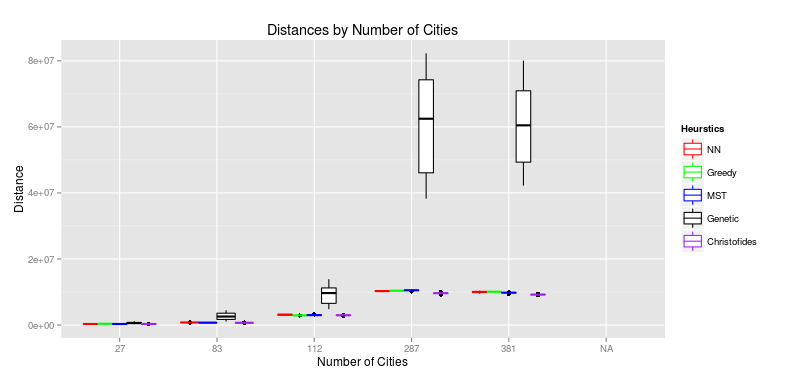
\includegraphics[width=.95\textwidth]{box_w_gen}
	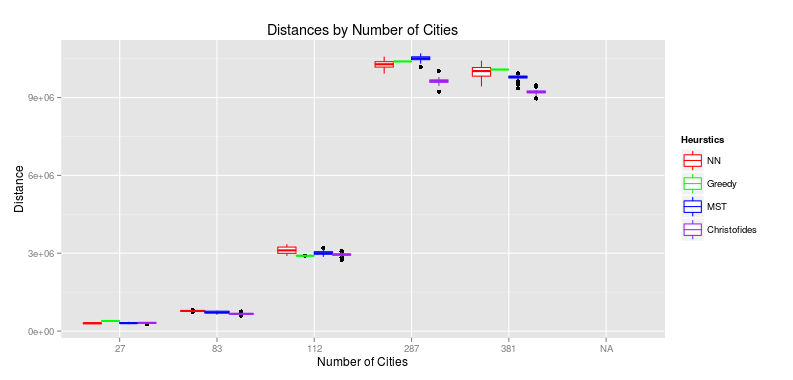
\includegraphics[width=.95\textwidth]{box_wo_gen}
	\end{center}
\end{figure}
\tab Upon inspecting these graphs it is clear to see that the algorithm that consistently finds the shortest distance is the Christofides algorithm. This is to be expected given the upper bound guarantees of distance that the heuristic provides. As for the second best algorithm, there seems to be a toss up in terms of distances between the various other heuristics. The two more consistent algorithms were the Minimum Spanning Tree (MST) and the Greedy Heuristic. In terms of actual average distance the Nearest Neighbor was comparable to both the MST and the Christofides heuristics. This suggests that the various approaches preform similarly and that the upper bound guarantees are a set of insurances but not a hard line for how the heuristic with preform in the real world. \\
\begin{figure}[t!]
	\begin{center}
	\caption{The top plot has all of the heuristics and the their runtime  and the bottom shows has all but their memory use.}
	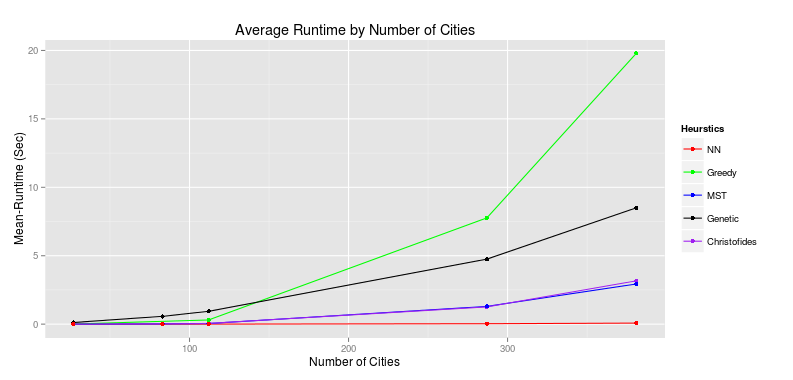
\includegraphics[width=.95\textwidth]{time_numcities}
	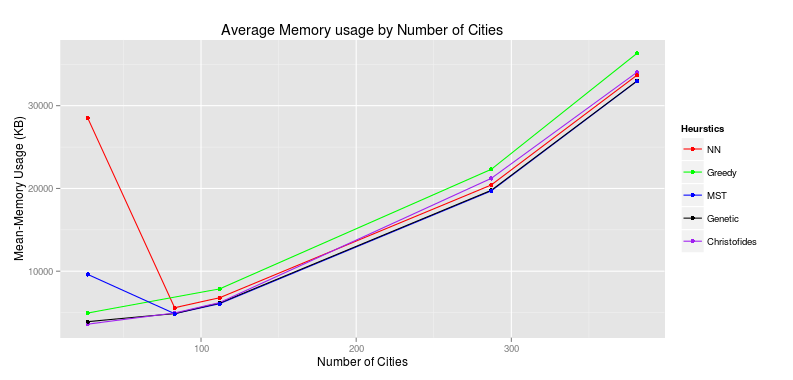
\includegraphics[width=.95\textwidth]{mem_numcities}
	\end{center}
\end{figure}
\tab Needless to stay there are more comparisons that need to be made to see how these heuristics preformed overall. The next set of graphs is based on the usage of the memory (in Kilobytes KB) and the time (in seconds) of each of the heuristics. For the sake of simplicity the mean average for the time and space measurement have been plotted on figure 5:2.\\
\tab For the amount of time that the heuristics run in there are a few interesting items to be observed. First is that Nearest Neighbor heuristic constantly has the lowest runtime and scales over the number of cities very well. This is particular since it means that with a single pass through the data that it finds a solution instead of having to do several extra functions at each iteration. As for the next two heuristics MST and Christofides, there is clearly more time used and this can be described two ways. The first is that the algorithmic complexities are higher than the NN approach by a factor of $\log(N)$. While this does not seem like a lot it clearly has an impact on the actual runtime of the heuristics. The Genetic heuristic by contrast took a lot of time. This comes from the constant number of iterations that heuristics always runs regardless if the heuristic as found a good solution or not. While in the long run the other heuristics should take more time than the offset of the constant but apparently for the states that were used in the test, this is not the case. This is interesting in that it means that there could be room for improving the stopping point of the Genetic heuristic. Finally, the other item that should be observed is the amount of time that it takes for the Greedy heuristic to run. The interest stems from the fact that the algorithmic complexity is $O(N^2)$ just like the Nearest Neighbor heuristic but takes vastly more time than Nearest Neighbor. This could be because the heuristic has to take more iterations to find the solution and for iteration checking the degrees and if a cycle is made. The fact that there are two steps in each iteration allows for extra amount of work that was not present in the other construction heuristics. It also is telling that the approach apparently expends the entirety of the number of iterations to find the solution hence the running times of the heuristics.\\
\begin{figure}[h!]
	\begin{center}
	\caption{The top plot has all of the heuristics and the their runtime times the distance and the bottom shows has all but their memory use times their distance.}
	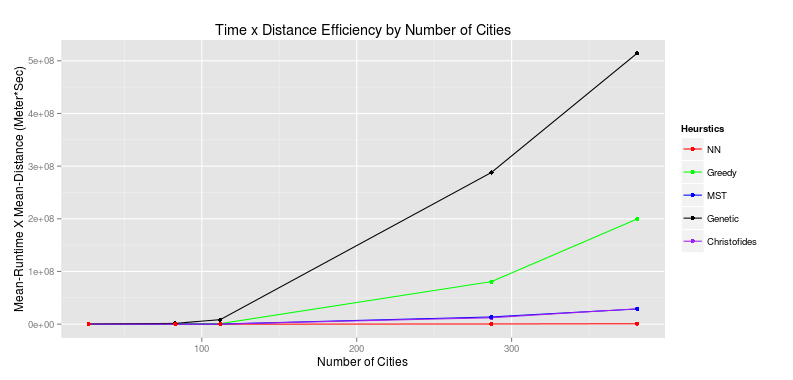
\includegraphics[width=.95\textwidth]{timexdistance_numcities}
	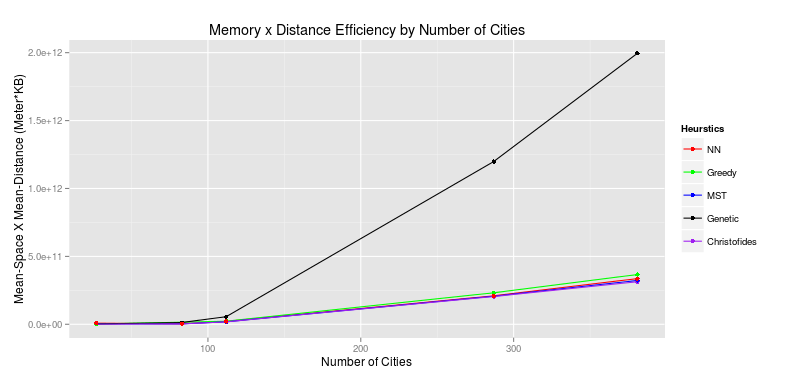
\includegraphics[width=.95\textwidth]{memxdistance_numcities}
	\end{center}
\end{figure}
\tab In regards to the memory usage the methods used were described in chapter 2, however the spikes in Nearest Neighbor and MST are anomalies that occurred with the first instance of running the heuristic. What is interesting here though is that the algorithmic space complexity is $O(N+E)$ or $O(N)$ for each of the heuristics and that the usage of memory conforms to this. This is seen through the slight parabolic curves of the the heuristics. The non linear curve could easily be explained by the amount of memory that the graph takes up for each heuristic $O(N^2)$. The consistent slope of each of these heuristics is due to the fact that the heuristics are all adding a similar amount to the memory usage as a whole. As for the early spikes in the Nearest Neighbor heuristic and the Minimum Spanning Tree heuristic, it can only be supposed that this phenomenon is due to the overhead of startup. That being said, there should be more investigation into this phenomenon, but in examining the individual characteristics it appears to be a single outliers that skews the whole mean. All and all, in terms of the memory usage all of the heuristics are similar enough to each other in terms of average value that there is not a clear advantage of one heuristic over the others.\\
\tab Figure 5:3 help bring the various heuristics into a sharper focus in terms of which are more useful in implementation than the others. By looking at the ratio of the distance and either the time or the memory usage for each heuristic. The result is that their is a greater separation of the heuristics than in the previous figures. The result of this separation allows for a more in depth inspection of the the various heuristics and their overall performance across multiple metrics. For instance, while the genetic heuristic is in the relatively similar position as in figure 5:1, the Greedy heuristic becomes distinct in looking at the product of time and distance. Interestingly, The other three heuristics are pretty similar to each other but with Nearest Neighbor having the best ratio of distance and time. In terms of memory and distance, with the exception of genetic heuristics the heuristics are pretty similar. The difference in the Genetic heuristic can be seen from the fact that the distances are on averaged significantly more than the others. Overall, it is clear that from an actual distance, runtime, and memory perspective that MST, Christofides, and Nearest Neighbor are the strongest heuristics.
\chapter{Conclusions}
\tab Overall, this paper only examines a small number of the possible implementations possible for the heuristics of the TSP. This paper set out to examine some of the heuristics of the TSP on real world data and examine how those heuristics preformed. The five states that were used based on the number of cities that hey contained to see how each of the heuristics scaled in terms of runtime and space. To ensure that the results were significant the results were processed using t-tests and then were graphed and analyzed to find trends in the heuristics' performances. In drawing final conclusions based on this process, it seems most appropriate to discuss each of their heuristics and their benefits and draw backs than the heuristics as a whole. Each of the heuristics are discussed in the order they were presented in chapter 3.\\
\tab The first heuristic that should be acknowledged is the Nearest Neighbor heuristic. This was both the simplest approach to intuitively understand and to implement. As an added bonus the overhead knowledge for this approach was minimal to say the least. The only theoretical downside to this approach was that it was not necessarily the most reliable in terms of the route it returns and the distances it finds. By the distances I mean that unlike some of the other heuristics there is no guarantee of a upper bound for the Nearest Neighbor. This is detrimental in the case of some route dependent companies such as UPS or FedEx since it means that for the drivers they can only hope that the route is good and not know that it is.\\
\tab In actual practice for the graphs that it was given, however, Nearest Neighbor preformed quite well in producing some of the shorter routes in less time and memory than the other heuristics. It was on par in terms of memory usage and distance and took the least amount of time to run. This meant that in the efficiency of the heuristic, the Nearest Neighbor was the most efficient heuristic in terms of time and space. Overall, combined with the ease of implementation, the Nearest Neighbor is a decent heuristic that's only drawback  is its lack of a distance guarantee. In short Nearest Neighbor is a decent approach but not the most reliable so it could be used as a basic starting point and an sanity check for testing other heuristics.\\
\tab The Greedy heuristic is the second construction heuristic that was examined in this paper. This was also a relatively simple heuristic that only required that the edges be sortable and that there are two functions that check to see if an edge that would be added would violate the constraints of the solution. The overhead was minimal though there were some basic graph theory knowledge or algorithms needed. Also, as in the case of Nearest Neighbor there is not a upper bound guarantee provided by the heuristic's approach.\\
\tab In implementing the Greedy heuristic, there were several issues in implementing the helper functions and the need to make the edges sortable was difficult at times. The difficulty came from the key idea to make sure that it would allow for a consistent pattern to account for the directed nature of the edges in the graph. The result of all of this extra work also showed in the poor runtime of the heuristic as well despite the algorithmic runtime from the heuristic. While the memory usage was on par with the other heuristics and the heuristic always provided a deterministic answer, it did not always provide a solution. This final part is detrimental to the usability of the Greedy heuristic. From looking at all of the various ways that heuristics are being judged in this paper, it is more useful for Nearest Neighbor in the place of the Greedy heuristic since it has all of the same theoretical benefits of the Greedy approach but providing the answer in less time and consistently finding an answer. As a result of the research of this paper, it is favorable to implement a different construction heuristic instead of the Greedy heuristic.\\
\tab The first of the more complex non-greedy approaches to TSP heuristics that was examined was the Minimum Spanning Tree heuristic. This was also the first heuristic that was examined that had an upper bound guarantee. This is a key point to focus on in the question for how these heuristics preform on real world data. The guarantee is what a company that wants to implement a heuristic would look at to make cost estimates and the better the guarantee the less cost that needs to be calculated. As a trade off, there is a increase of the knowledge that is needed for the implementing of the Minimum Spanning Tree heuristic as well as a few new classes needed and the increase in algorithmic complexity compared to the Nearest Neighbor and Greedy heuristics. Like the Nearest Neighbor heuristic though there is not a deterministic approach that would yield and consistent answer 100\% of the time. Also, the MST required the edges to be sortable though not as strictly as the Greedy heuristic. These minor trade offs are definitely worth it however in looking at the performances and the scalability of the MST heuristic. MST consistently was one of the best preforming routes in terms of time, space and distance.\\
\tab There were several different ways that this heuristic could have been implemented despite the simple unintuitive approach that it took. The extra classes that were needed including trees and the nodes for the trees though this did not increase the memory usage as much as one would expect. With the implementation that was used in this paper, there is room for improvement in later work and experimentation. In the implementation it was difficult to ensure that the tree was being built correctly for instance. However, the result of this extra work was a consistent algorithm that preformed comparably to the others in terms of distance and memory and while not as good in terms of time as the Nearest Neighbor, scaled well. As a solid starting point to allow for some insurance, MST is a relatively good algorithm to implement and preforms well as the theoretical work would have us believe.\\
\tab In every form of analyzing heuristics in this paper, Genetic heuristics show all of the signs of not being usable in actual implementation. If anything this shows the complexity and difficulty in implementing a Genetic algorithm efficiently and correctly. It should be noted that for the smaller number of cities the Genetic algorithm preformed almost as well as the other heuristics. The major flaw of this heuristic was in the lack of scalability of the heuristic in its performance. Some of this is due to the complexity of the heuristic but also to the idea that genetic heuristics could operated better in parallel. However, such as investigation was outside of the scope of this paper. It is also to be noted that while the distances and implementation complexity for Genetic heuristics were the greatest that the memory and runtime were not by any stretch the worst among the heuristics.\\
\tab Before ruling out the possibility of Genetic algorithms as a viable option, there should be more research done on the various techniques that could be used to improve the reliability of Genetic heuristics. Some improvements and possible areas of research could include, using other heuristics to gather the population for improvement, the various effects of mutation on the routes, breeding approaches, inheritance algorithms, and experimentation into the number of iterations the heuristic should run. It is important to note that Genetic heuristics fall under the category of tour optimization heuristics, hence it only improves what you give it and in this case with the implementation of giving random cities it is unsurprising that poor results are returned. As a final note, the Genetic heuristics could be a good set of heuristics to examine further but the current implementation would not be preferred over most other approaches.\\
\tab The final and most complex heuristic that was examined in this paper is the famous Christofides heuristic. This as mentioned earlier was one of the more complex than the other heuristics in terms of the knowledge that was needed to implement the heuristics. However, some of this was mitigated by the work on the MST heuristic. Also the Christofides heuristic has the worst algorithmic complexity of the heuristics with a time of $O(N^3)$ as a trade off for having the best upper bound of all of the heuristics with the maximum distance only being $3/2$ times the optimal length. In addition to this as a added bonus there is a bonus of having a space usage as good as the other heuristics of $O(N)$.\\
\tab The results of the tests reflect the upper bounds and the space usage found in theory. The space usage is on par with the other heuristics and the distances were universally both the shortest and the second most consistent. In terms of overall efficiency of time and space in regards to distance the Christofides heuristic preformed similarly to the MST heuristic which is not surprising giving the similarity in the algorithmic complexities and spaces. The key part of the Christofides heuristic is the guaranteed upper bound for the results produced. This means that there isles to worry about in terms of calculating potential cost of taking a sub-optimal route since the amount that the route would be off is significantly less than with the other heuristic approaches. In terms of the complexity of implementation, it was key to ensure that the algorithm for finding the Euler cycle was correct as well as the construction of the Euler graph. In short, in terms of theory, the Christofides heuristic is the best heuristic to use if one can implement the helper functions correctly and on real world data preforms better than expected in some cases.\\
\tab For each heuristic, there is room for improvement. These improvements range in size and complexity from the smaller and more subtle changes it the use of one heuristic over another or even to a complete rethinking of the approach to take. For future work other heuristics and approaches should definitely be considered beyond the construction heuristics examined as well as a dedicated study to the Genetic heuristics. Also, questions on running an ensemble of heuristics in parallel could also be an interesting line of study presenting an approach that attempts to combine the best of all worlds.\\
\tab In terms of how each of these heuristics preformed on the real world state data, it is clear that while considering theory is important for the choice of heuristic, it should not be the sole driver of the choice. For instance the Nearest Neighbor with no guarantee was one of the most efficient approaches while its most similar counter-part the Greedy heuristic preformed poorly. That being said, in regards of the best distances it is clear to use at least the MST heuristic if not the Christofides heuristic for their guarantees of performance but with time Nearest Neighbor out preforms all of the other heuristics examined in this paper. To be safe it is good to have both Nearest Neighbor and the Christofides heuristic for comparison and reliability. 

\appendix
\chapter{The Use of Java}
\tab Java is the language that is used for this project. Java is it is an Object Oriented Programming language that uses an abstraction called a Virtual Machine to run its code instead of the computer itself. This allows for code that is written on one kind of system to be run on other kinds of systems as long as they all have a compatible version of Java (and thus the Java Virtual Machine or JVM) on them. The choice to use Java is mainly due to its platform independent nature for the implementation for each heuristic. In addition to Java the other languages considered for this project were NetLogo, Python, or C++. NetLogo is a simple multi-agent based language and as such is not suited to the flexible implementation of TSP heuristics or in the gathering of data needed to draw necessary conclusions. Python is a simple interpreted language that would be easy to implement the heuristics with but also can lack the durability of other languages as well as support and use in the workforce for large scale projects where efficiency of the heuristics becomes key.  While C++ might be easier to examine the memory usage and is also faster, it is dependent on the system that the heuristic that is running on. C++ also lacks some of the durability of Java making it less than ideal for larger problems and individual efforts such as this to create heuristics. As a result of these different factors, Java, while not the fastest language not only abstracts from the machine's system but also provides the durability of for a individual endeavor and for instances of large datasets at the cost of some difficulty in extracting memory usage. This difficulty is to be expected because of the fact that Java programs run on the JVM instead of the Computer itself. The reason this drawback is a fair trade-off is that it avoids any issues with questions regarding code dependency on one specific operating system or about questions of efficiency based on the system itself. Another reason for using Java is that several companies that depend on these heuristic algorithms also use Java. Part of the purpose of this project is to test the implementation capabilities and as such choosing Java was done with the fact that several organizations whose services require a fast an efficient solution to TSP would also use Java as their main development language. Java is  used to both parse the data files as well as the visualization of the graph and pathways. Each of the experiments will also be written and run Java naturally. For clarity in each heuristic will then  be displayed in both their pseudo-code format as well as their implementation in Java in addition to the  explanation. Having said all of this, the purpose of this paper is not to argue the implementation in one language over another but instead to focus on the implementation of heuristics for the TSP.\\

\bibliography{Thesis}

\end{document}